\section{Backbone architecture search}
\label{sec:appendix-backbone-search}

The backbone we use was selected through two phases of search.

\paragraph{Encoder.} The first phase compared five encoder variants
holding the rest of the backbone fixed: a TiDE-style residual MLP, a
wider MLP variant, a TimeFM-style residual SiLU block, a 1-D
convolution, and a bidirectional GRU. The bidirectional GRU won by a
wide margin, with roughly a $62\%$ relative increase in the
contrastive gap over the MLP baseline at $50$k steps. Each patch is
read as a sequence of $W$ scalar timesteps, which gives the GRU
access to the local temporal structure that an MLP collapses into a
single linear projection.

\paragraph{Forecaster.} The second phase varied the transformer
block. The depthwise causal convolution of Section~\ref{sec:forecaster}
is essential: removing it drops the converged gap by roughly $20\%$. A
feed-forward multiplier of $4$ outperforms $2$ by a few percent. GELU
outperforms SiLU at the same parameter count. Doubling the number of
attention heads from $8$ to $16$ gave no measurable gain.

\paragraph{Depth.} We compared $L \in \{12, 16, 20\}$ at $H = 1024$.
At $200$k steps the $16$L variant led; the $20$L variant trained more
slowly and lagged behind early on. After the full $2$M steps, the
$20$L matched the $12$L on the contrastive gap but came out slightly
worse on recovery ($6.77$ vs $6.96$). We attribute this lag to
imperfect learning-rate scaling for the deeper model rather than to a
depth-vs-shallow finding, and use $L = 12$ throughout our runs as
the compute-efficient choice that does not lose recovery quality.

Figure~\ref{fig:training-gap} shows the training gap trajectories for
the $12$L and $20$L variants over the full training run.
Figure~\ref{fig:depth-comparison} shows the $200$k snapshot
comparison across $L \in \{12, 16, 20\}$.

\begin{figure}[t]
  \centering
  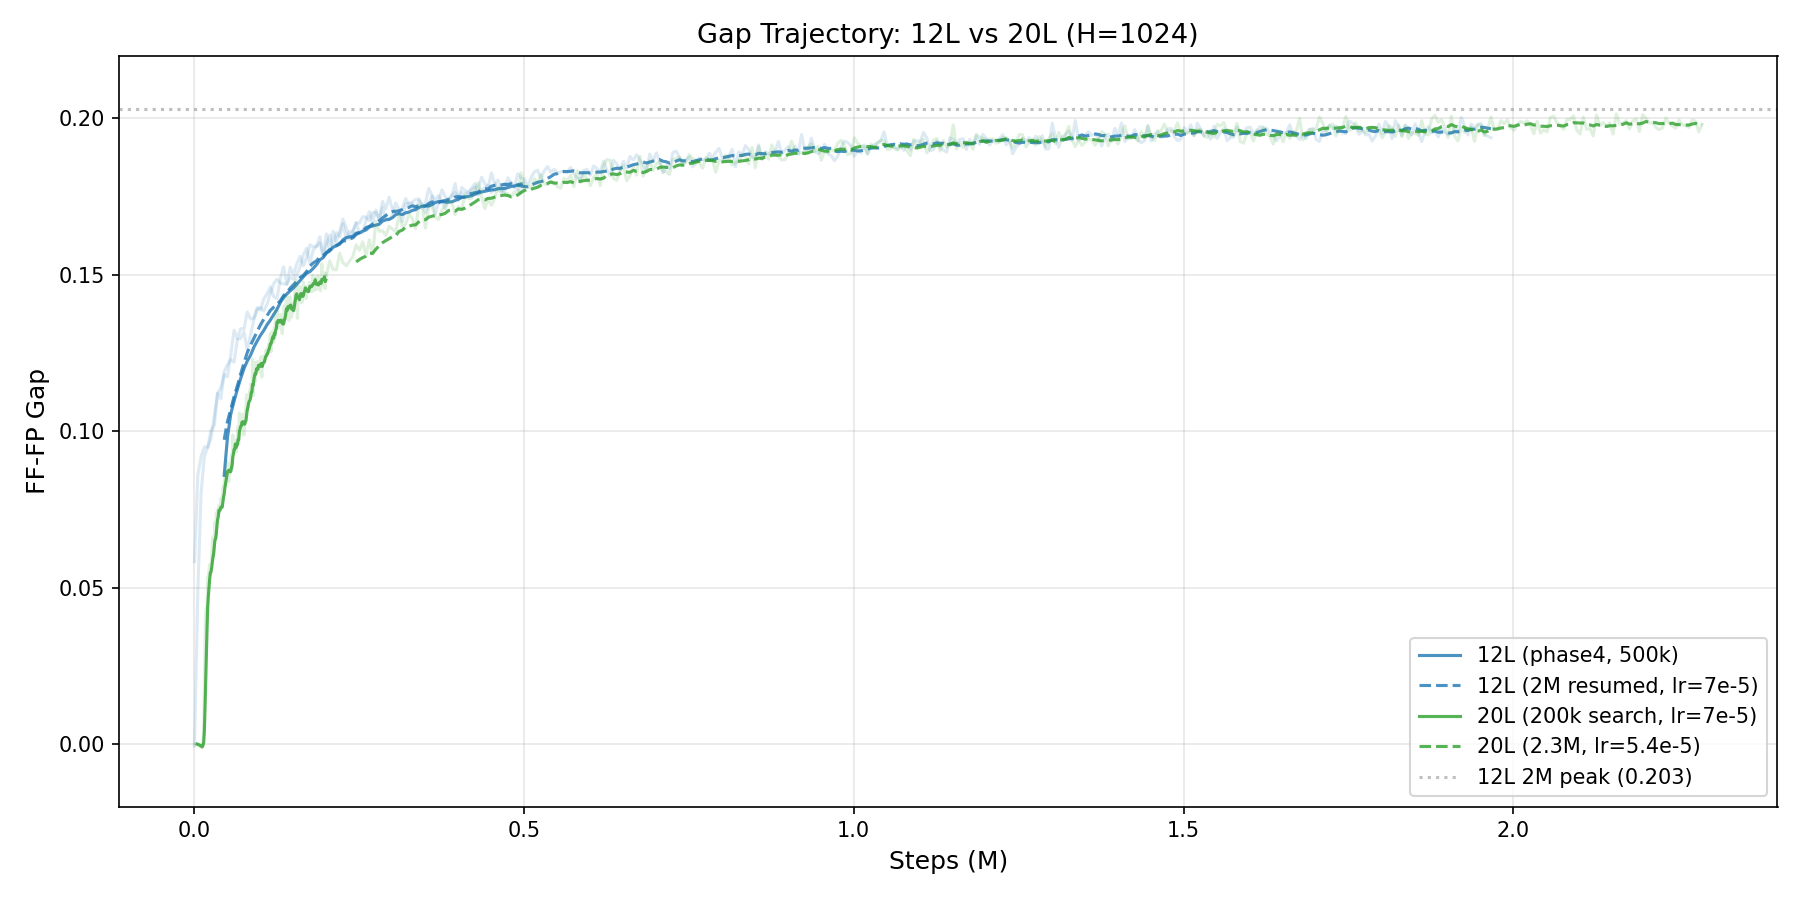
\includegraphics[width=0.85\linewidth]{figures/training_gap_full.png}
  \caption{Contrastive gap (forecast--future minus forecast--past) over
    training steps for the $12$L (extended to $2$M steps) and $20$L
    (extended to $2.3$M steps) backbones at $H = 1024$.}
  \label{fig:training-gap}
\end{figure}

\begin{figure}[t]
  \centering
  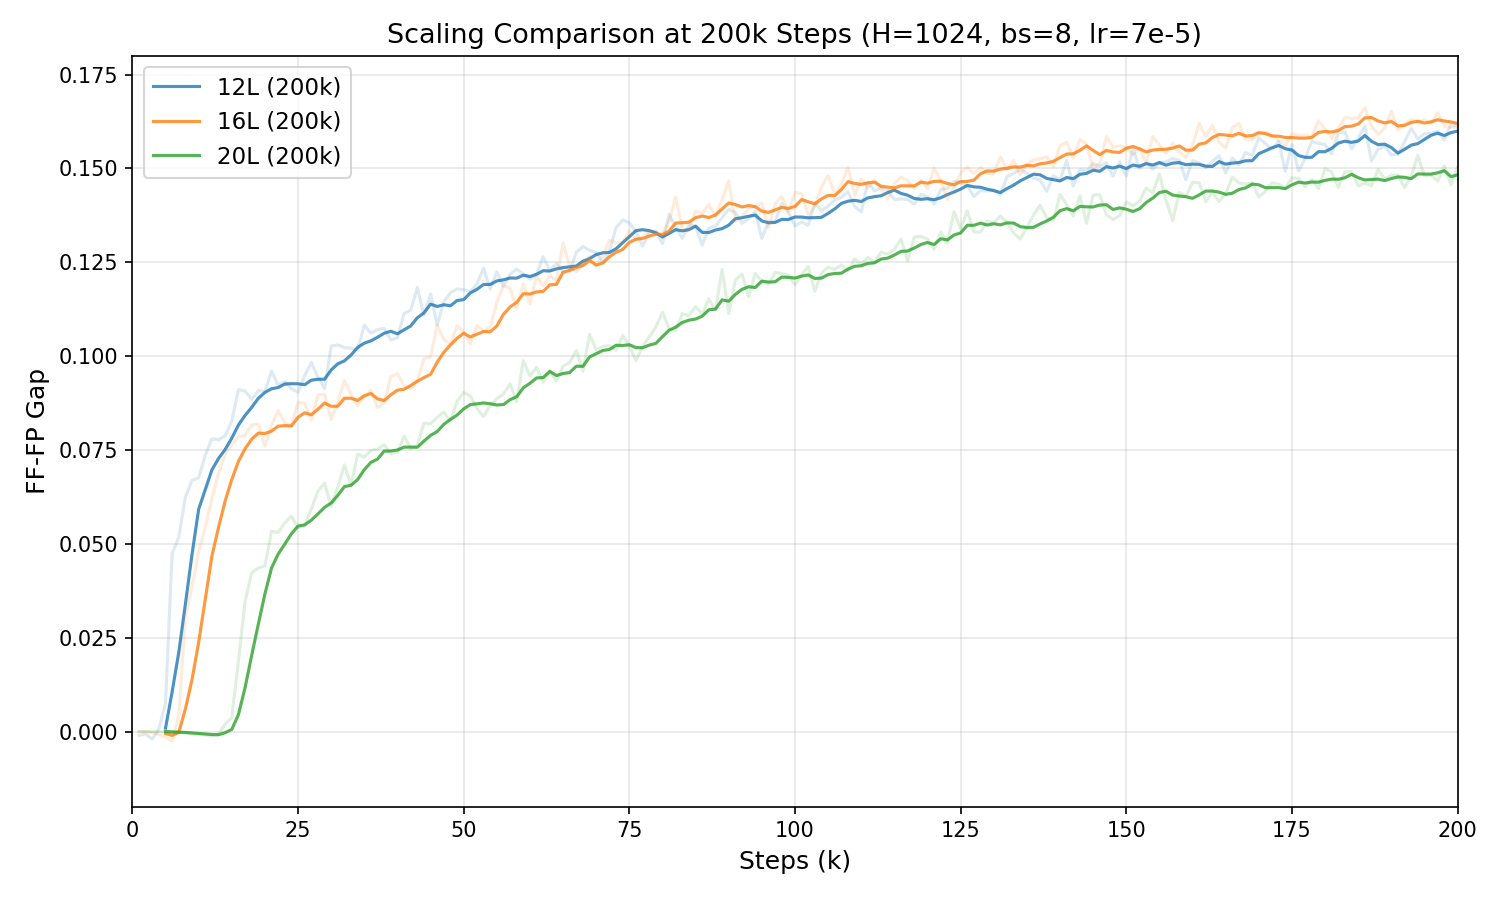
\includegraphics[width=0.7\linewidth]{figures/training_gap_depth.png}
  \caption{Contrastive gap at $200$k training steps for $L \in \{12,
    16, 20\}$ at $H = 1024$.}
  \label{fig:depth-comparison}
\end{figure}
